\documentclass{report}
\title{Radio Collar Tracker Post-Processing Manual}
\author{Nathan Hui, Project Lead\\Engineers for Exploration, UC San Diego}
\date{\today\\v0.1}
\usepackage{fullpage}
\usepackage{hyperref}
\usepackage{mdframed}
\usepackage{graphicx}
\usepackage{textcomp}
\usepackage{moreverb}
\hypersetup{
    colorlinks,
    citecolor=black,
    filecolor=black,
    linkcolor=black,
    urlcolor=blue
}
\begin{document}
\maketitle
\tableofcontents
\chapter{Processing Steps}
	To process data from the Radio Collar Tracker drone, follow the below steps:
	\begin{itemize}
		\item Boot the laptop into the Macintosh partitition.
		\item Insert the USB data drive into the laptop.
		\item Use the ``PostProcessing'' command on the Desktop to start the post-processing program.
		\item Select the desired run when prompted.
		\item If prompted, enter the run number.
		\item If prompted, enter the flight altitude.
		\item If prompted, enter the target collars.
		\item When the program is processing, the command line window will have a progress bar to show progress.
		\item When the program finishes, open the run folder.
		\item Open all of the images in the run folder.  The filename will be similar to RUN\_010006\_COL\_000001.png.  The first number is the run number, and the second number is the collar number.
		\item Select the image that shows the brightest peak.  You should be looking for a graph with the largest range in the scale bar.  The correct image should also have a peak with data that falls off cleanly, such as in Figure \ref{fig:reference_plot}.  The peak should be at least 3 dB difference from the rest of the data.
			\begin{figure}[ht]
				\centering
				\caption{Reference Plot Showing Ideal Peak}
				\label{fig:reference_plot}
				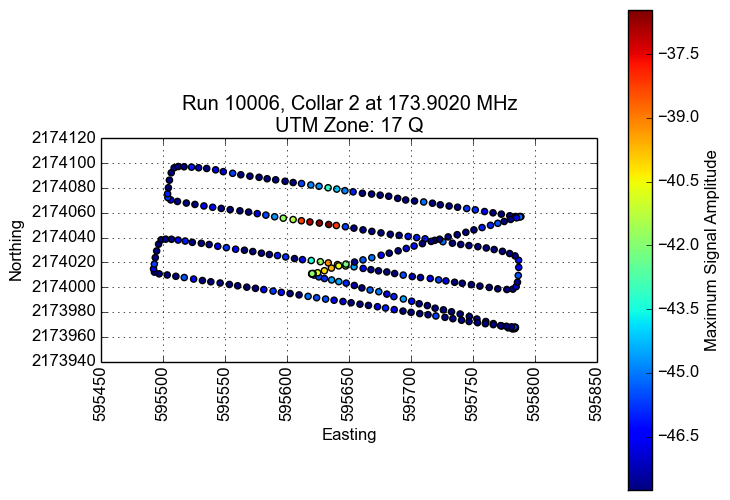
\includegraphics[width=\textwidth]{RUN_010006_COL_000002.png}
			\end{figure}
		\item Use the ``makeShapefile'' command on the Desktop to start the shapefile generation program.
		\item Select the .csv file corresponding to the image you selected earlier.  The filename should be exactly the same except for the file extension.
		\item Save the shape file in an eaily accessible location.
		\item Open QGIS.
		\item Create a new vector layer by selecting Layer \textrightarrow Add Layer \textrightarrow Add Vector Layer.
		\item Select the shape file you saved earlier.
		\item Use QGIS to create an interpolation over the vector layer by selecting Raster \textrightarrow Analysis \textrightarrow Grid (Interpolation).  Set the interpolation variable to the ``measurement'' field, and save the output TIFF file to a reasonable location.  You can modify the interpolation settings to adjust the smoothness and coverage of the interpolation.
		\item If the TIFF has not been automatically loaded into QGIS, load it by selecting Layer \textrightarrow Add Layer \textrightarrow Add Raster Layer.
	\end{itemize}
\chapter{Modifying Existing Run Configurations}
	\section{Changing the Run Number}
		\begin{itemize}
			\item Open the RUN file in the run you are trying to modify in a text editor.
			\item Change the RUN file to have the line in Figure \ref{lst:RUN_file}
				\begin{figure}[ht]
					\centering
					\caption{RUN File Contents}
					\label{lst:RUN_file}
					\begin{listing}{1}
run_num: 123456\end{listing}
				\end{figure}
			\item Save the RUN file.
		\end{itemize}
	\section{Changing the Flight Altitude}
		\begin{itemize}
			\item Open the ALT file in the run you are trying to modify in a text editor.
			\item Change the ALT file to have the line in Figure \ref{lst:ALT_file}.  The flight altitude should be in meters above ground level.
				\begin{figure}[ht]
					\centering
					\caption{ALT File Contents}
					\label{lst:ALT_file}
					\begin{listing}{1}
flt_alt: 30\end{listing}
				\end{figure}
			\item Save the ALT file.
		\end{itemize}
	\section{Changing the Collar Definitions}
		\begin{itemize}
			\item Open the COL file  in the run you are trying to modify in a text editor.
			\item Change the COL file to have the desired collars, one on each line, as shown in Figure \ref{lst:COL_file}.  The collar frequencies should be in Hertz.
				\begin{figure}[ht]
					\centering
					\caption{COL File Contents}
					\label{lst:COL_file}
					\begin{listing}{1}
1: 123456789
2: 234567890
3: 345678901\end{listing}
				\end{figure}
			\item Save the COL file.
		\end{itemize}
\end{document}
